\documentclass[conference]{IEEEtran}
\usepackage[utf8]{inputenc}
\usepackage{amsfonts}
\usepackage{caption}
\usepackage{graphicx}
\usepackage{listings}
\lstset{
    basicstyle=\tiny\ttfamily,
    keywordstyle=\color{blue}\ttfamily,
    stringstyle=\color{red}\ttfamily,
    commentstyle=\color{green}\ttfamily,
    breaklines=true
}
\usepackage{url}

% correct bad hyphenation here
\hyphenation{op-tical net-works semi-conduc-tor}

\begin{document}
\title{Relatório - EP3}

\author{\IEEEauthorblockN{Tiago Koji Castro Shibata - 8988730}
\IEEEauthorblockA{Escola Politécnica\\
Universidade de São Paulo\\
tiago.shibata@usp.br}
}

\maketitle

\section{Introdução}
Esse relatório acompanha o terceiro exercício programa (EP3) da disciplina PCS3556 - Lógica Computacional. Nesse exercício programa, é implementado um simulador de autômato finito determinístico e não determinístico em Elixir.

\hfill 26 de Março de 2018

\section{Tarefa}

A tarefa consiste em implementar um algoritmo de simulação de autômato determinístico e não determinístico em Elixir, experimentando com conceitos vistos em aula.

Um autômato finito é definido pela tupla:

\begin{equation}
M = (Q, \Sigma, \delta, q_0, F)
\end{equation}

Onde $Q$ é a lista de estados do autômato, $\Sigma$ o alfabeto de entrada, $\delta$ a função de transição, $q_0$ o estado inicial, e $F$ o conjunto de estados de aceitação. Dado um autômato, estado inicial e cadeia, o algoritmo deve retornar se é possível que o autômato aceite a cadeia (ou seja, há uma sequência de transições iniciando no estado inicial e acabando em estado de aceitação que gere a cadeia desejada).

Como vimos em aula, o estudo de autômatos é bastante importante. Linguagens reconhecidas por autômatos são regulares, e toda linguagem regular pode ser representada por um autômato. Autômatos determinísticos (DFA) e não determinísticos (NFA) são equivalentes (é possível converter qualquer NFA em DFA equivalente, que aceita e rejeita as mesmas cadeias; no entanto, para um NFA de $n$ estados, o DFA equivalente pode ter até $2^n$ estados, portanto a representação em NFA pode ser mais conveniente. No entanto, a simulação de DFA é muito mais fácil, já que não há várias transições possíveis a se testar).

Na hierarquia de Chomsky, autômatos finitos estão na classe de linguagens regulares:

\begin{minipage}{\linewidth}
    \centering
    \label{chomsky}
    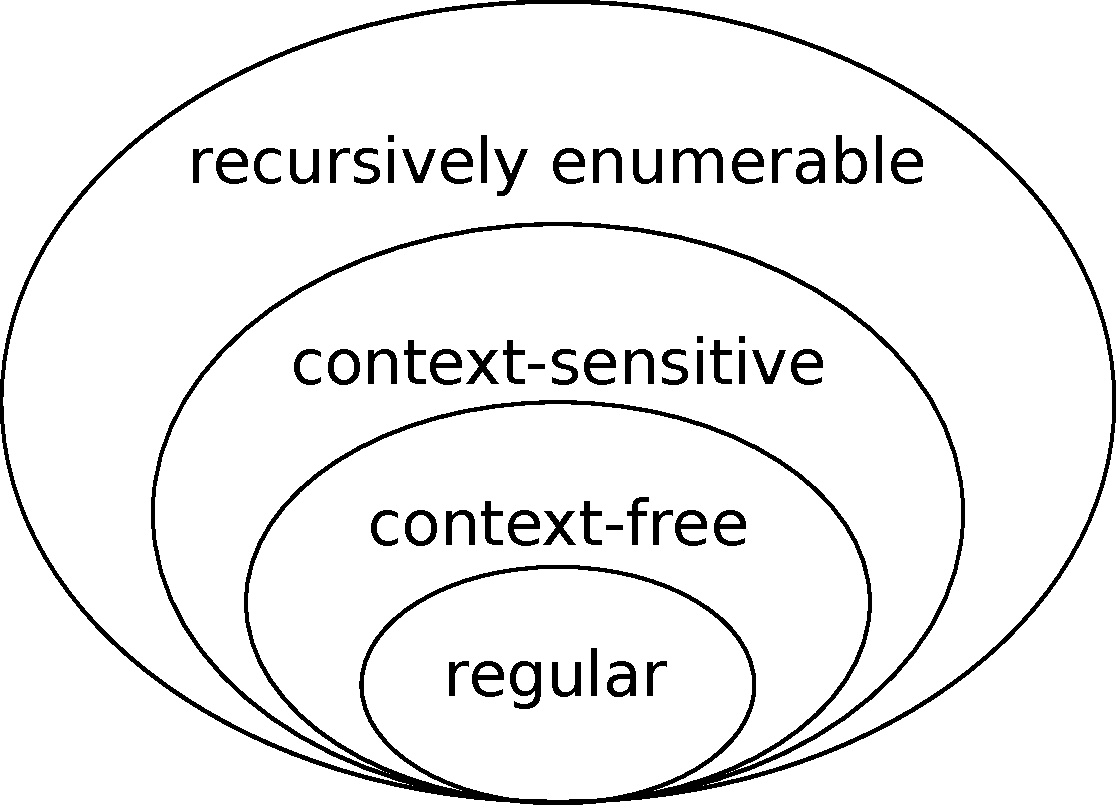
\includegraphics[width=0.8\textwidth]{Chomsky-hierarchy.pdf}
    \captionof{figure}{Hierarquia de Chomsky}
\end{minipage}
\\

Nessa implementação, $\delta$ é dado como uma lista de transições (lista de tuplas do tipo $\{estado, caractere, pr\acute{o}ximo\_estado\}$, significando que $\delta(estado, caractere) = pr\acute{o}ximo\_estado$). Os estados de aceitação são dados como uma lista de estados e a cadeia desejada é dada como uma lista de elementos.

\section{Estruturas de dados}

Em alguns locais, estruturas de conjunto fornecidas pelo Elixir (\emph{MapSet} foram usadas. O uso de conjunto evita que varramos a lista toda para buscar um elemento, e o conjunto permite operações fáceis e rápidas de união ou diferença quando necessário. Funções do módulo \emph{Enum} foram usadas para facilitar a programação funcional.

\section{Algoritmo}

O algoritmo deve suportar autômatos não determinísticos, incluíndo transições vazias. O uso de transições vazias adiciona uma dificuldade à tarefa: ao seguir uma sequência de transições, o algoritmo deve acompanhar estados visitados para não ficar preso em um ciclo de transições em vazio.

A função \emph{next\_state} calcula os possíveis próximos estados dado o estado atual, regras de transição e caractere atual. Para evitar ciclos infinitos em caso de transição vazia, os estados já vistos são mantidos em um conjunto; o estado não é visitado novamente se já pertencer ao conjunto. A função filtra regras que iniciam no estado inicial e transitam pelo caractere na entrada. Ela também se chama recursivamente por transições vazias, e concatena os resultados. Finalmente, é usado um \emph{pipe} para um \emph{MapSet}, removendo quaisquer estados repetidos:

\lstinputlisting{1.ex}

Os testes foram essenciais no desenvolvimento, já que essa função apresenta alguns \emph{corner cases}, como ciclos de transições vazias. A função foi testada com um autômato com ciclo de transições vazias e funcionou corretamente:

\lstinputlisting{1_test.ex}

A função \emph{final\_states} computa os possíveis estados finais de um autômato não determinístico. Ele recebe o estado inicial, sentença de entrada e regras de transição, e retorna estados finais possíveis consumindo um caractere por vez e chamando-se recursivamente:

\lstinputlisting{2.ex}

A função foi testada:

\lstinputlisting{2_test.ex}

A função \emph{accepts\_sentence?} verifica se uma sentença pode ser aceita por um NFA. Para isso, a função recebe uma lista de estados de aceitação, e busca por intersecção com os estados retornados por \emph{final\_states}:

\lstinputlisting{3.ex}

Finalmente, foram feitos testes de \emph{accepts\_sentence?}:

\lstinputlisting{3_test.ex}

\section{Resultados}

A implementação foi um sucesso e passou nos testes realizados. Casos com transições vazias, incluindo ciclos, foram testados e aprovados, e o código funcionou em qualquer DFA ou NFA testado.

\section{Conclusão}

Pude aplicar os conhecimentos da disciplina em um problema prático e realizar reconhecimento de cadeias usando autômatos finitos, uma das opções para reconhecimento de linguagens regulares. Pude aplicar conhecimentos de gramáticas e hierarquia de Chomsky na resolução de um problema em Elixir. A implementação foi, inesperadamente, bastante menos trabalhosa que a do exercício programa passado (EP2).

\begin{thebibliography}{1}
\bibitem{elixir}
Friedel Ziegelmayer. \emph{Elixir ExDoc}. \url{https://hexdocs.pm/elixir/}, acessado em 11/02/2018
\end{thebibliography}

\end{document}
